\documentclass{article}

\usepackage{blindtext}
\usepackage{graphicx}
\usepackage{caption}
\usepackage{subcaption}
\usepackage{float}
\usepackage[toc,page]{appendix}
\usepackage[margin=0.5in]{geometry}

\restylefloat{figure}

\graphicspath{ {./images/} }



\author{Oskar Mampe: 201368087}
\date{\today}
\title{Convolutional Neural Networks}


\begin{document}
    \maketitle
    \tableofcontents

    \section{Part I: Experimenting with Features}


    Firstly, for my experiments, I have tested various number of layers to see how it affects the performance of the network, changing it from the original 3 layers. Furthermore, I have decided to test the performance of different filter size's of the last convolutional layers.  I have decided to choose different kernel size, as to see whether the change in kernel size will have a positive affect by capturing larger, more complex features.\\


    \subsection{Implementation Decisions}

    When implementing the 2-layer model, I have deleted the last convolutional layer that took in 24-dimensional input and outputted a 32-dimensional output, as that seems the most reasonable jump from 16-dimensional output from the first convolutional layer.\\

    For the networks with more than 3 convolutional layers, in order to stay consistent, I have decided to follow the linear sequence of increasing the input layer by 8. Therefore, the third layer spits out a 32-dimensional tensor and the fourth layer will then output a 40-dimensional tensor. This also allows the model to train faster, as a larger difference between input and output will take significantly more time. Having to train 8 models takes significant amount of time without time-consuming features. There is an argument that doubling the input for the output features increases the accuracy, however in my experiment all 4 experiments follow the same sequence, so having a layer that does not follow the sequence will skew the results.\\

    For the kernel sizes, I have decided to follow the sequence 3, 5, 7, 9. Generally speaking, I wanted to see what effect the larger kernel sizes would have on the network. I have decided to start at 3 as it seems to be the lowest one used in literature.\\

    I have trained for 10 epochs, just as in the original model.

    \subsection{Results}
    \begin{figure}[h!]
        \centering
        \begin{subfigure}[t]{0.45\textwidth}
            \centering
            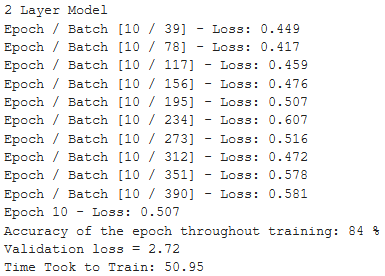
\includegraphics[width=0.6\textwidth]{2Layer_train}
            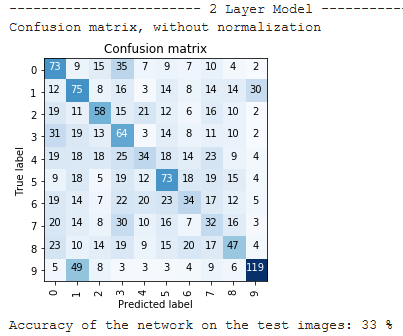
\includegraphics[width=0.6\textwidth]{2Layer_cm}
            \caption{2 Layer Network}
        \end{subfigure}
        \begin{subfigure}[t]{0.45\textwidth}
            \centering
            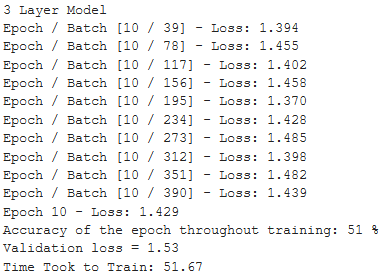
\includegraphics[width=0.6\textwidth]{3Layer_train}
            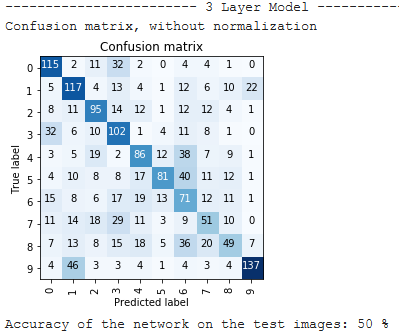
\includegraphics[width=0.6\textwidth]{3Layer_cm}
            \caption{3 Layer Network}
        \end{subfigure}
        \begin{subfigure}[t]{0.45\textwidth}
            \centering
            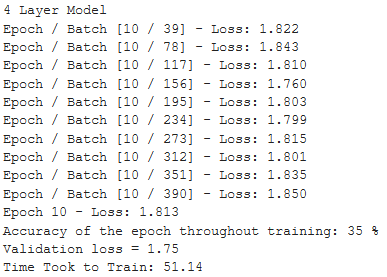
\includegraphics[width=0.6\textwidth]{4Layer_train}
            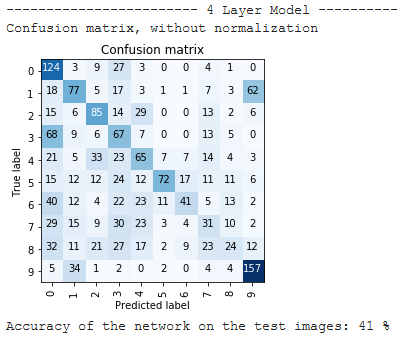
\includegraphics[width=0.6\textwidth]{4Layer_cm}
            \caption{4 Layer Network}
        \end{subfigure}
        \begin{subfigure}[t]{0.45\textwidth}
            \centering
            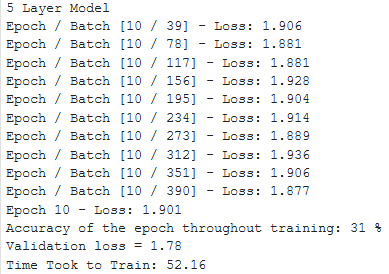
\includegraphics[width=0.6\textwidth]{5Layer_train}
            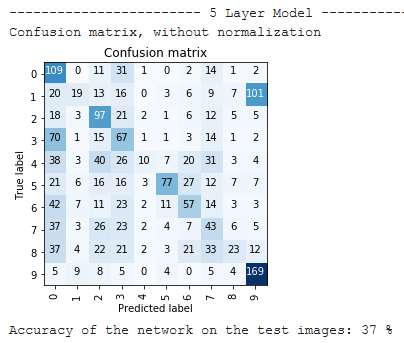
\includegraphics[width=0.6\textwidth]{5Layer_cm}
            \caption{5 Layer Network}
        \end{subfigure}
        \caption{Confusion Matrices for the Different Layers}
    \end{figure}
    \newpage
    \begin{figure}[h!]
        \centering
        \begin{subfigure}[t]{0.45\textwidth}
            \centering
            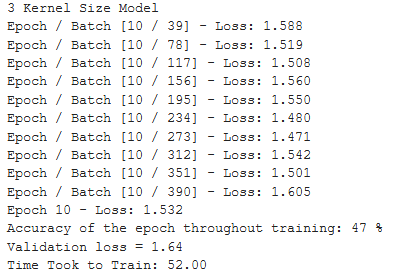
\includegraphics[width=0.6\textwidth]{3KS_train}
            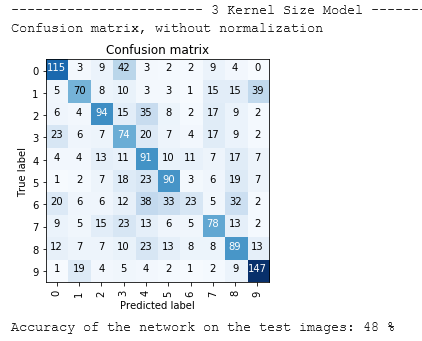
\includegraphics[width=0.6\textwidth]{3KS_cm}
            \caption{3 Filter Size Network}
        \end{subfigure}
        \begin{subfigure}[t]{0.45\textwidth}
            \centering
            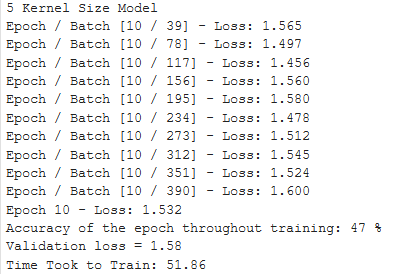
\includegraphics[width=0.6\textwidth]{5KS_train}
            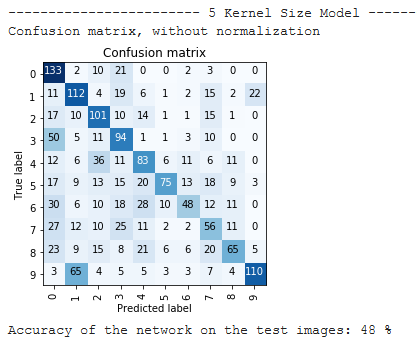
\includegraphics[width=0.6\textwidth]{5KS_cm}
            \caption{5 Filter Size Network}
        \end{subfigure}
        \begin{subfigure}[t]{0.45\textwidth}
            \centering
            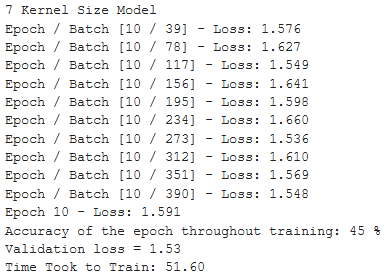
\includegraphics[width=0.6\textwidth]{7KS_train}
            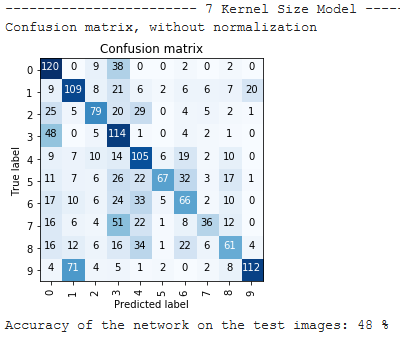
\includegraphics[width=0.6\textwidth]{7KS_cm}
            \caption{7 Filter Size Network}
        \end{subfigure}
        \begin{subfigure}[t]{0.45\textwidth}
            \centering
            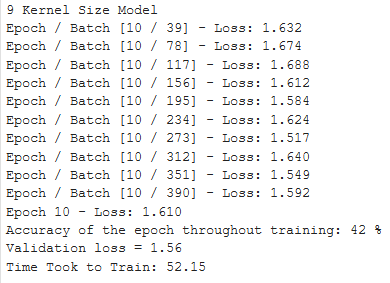
\includegraphics[width=0.6\textwidth]{9KS_train}
            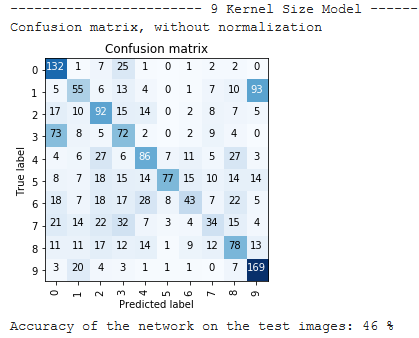
\includegraphics[width=0.6\textwidth]{9KS_cm}
            \caption{9 Filter Size Network}
        \end{subfigure}
        \caption{Confusion Matrices for the Different Layers}
    \end{figure}

    \subsection{Effect on Performance}
    There were several differences, that occurred after tweaking the features, as seen above.\\

    Firstly, the obvious effect can be seen in the 2 layer model where the training loss is very low, amassing a $80\%+$ accuracy. However, looking at the validation loss, and the confusion matrix, reveals that this high accuracy was only reached whilst training, leading to the conclusion that the model simply overfitted the data. The effect of that is that the model is not very good, since the model adjusted to the detail and noise of the data, therefore training weights that are optimised to this set of data. Hence, the 2 layer model could not take a random set of pictures and predict with an $80\%+$ accuracy.\\

    Another issue is that saving the lower layers' weights takes more space in terms of hard disk space, with the 2-layer model weights taking $180MB+$. This is an disadvantage, as a validation set is very useful metric to see whether the model is converging. Once an epoch, the model's weights could be saved. Then, when the training loss and validation loss are diverging, the model can be loaded from the previous save, where the validation loss was acceptable. Saving a 2-layer model can be quite memory intensive.\\

    Furthermore, higher number of layers seem to have the opposite problem of the 2-layer model, where the training loss is poor, but the validation loss is better. This might mean that the model takes a very long time to converge, and possibly require more than 10 epochs before any noticeable change is seen.\\

    As for the different kernel sizes, the difference in testing and training performance is minute. The worst performers were kernel size 7 and 9, where the data was seemingly overfitting, having a higher test accuracy than validation accuracy. However, they all seemed to hover at around about $48\%$, expect for kernel size 9, which is at $42\%$. This can be somewhat counter-intuitive as a higher number of kernel size should capture bigger and more rich features, but the model seems to preffer smaller features. This is probably due to some objects having small differences, for example, the difference between a cat and a dog are due to small features like ear shape etc.\\

    The training time required for each model seemed to be around about 52 seconds per epoch, without any model deviating from that pattern.\\

    The overall best performer was the original network with 3 layers and 4 kernel size. It seems to have the best balance in terms of not having too much layers and output sizes that it takes a very long time to train, and not overfitting, as it performed admirably in both validation and training.

    \section{Part II: Visualising Filters}

    \subsection{Implementation}

    I have implemented the filter visualisations by taking the weights of the first convolutional layer and showed it using plt.imshow(). However, I have used transforms.ToPILImage(), as normalising with pytorch.norm() didn\'t have noticeable effect, since the values were still very low and any change in them was not noticeable.

    \subsection{Results}
    \begin{figure}[h!]
        \centering
        \begin{subfigure}[t]{0.8\textwidth}
            \centering
            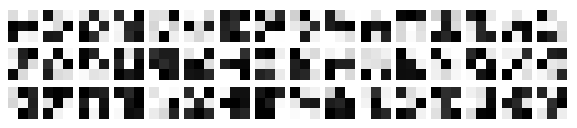
\includegraphics[width=0.8\textwidth]{Filters_before}
            \caption{Filters before training}
        \end{subfigure}
        \begin{subfigure}[t]{0.8\textwidth}
            \centering
            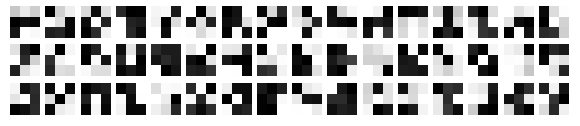
\includegraphics[width=0.8\textwidth]{Filters_during}
            \caption{Filters during training}
        \end{subfigure}
        \begin{subfigure}[t]{0.8\textwidth}
            \centering
            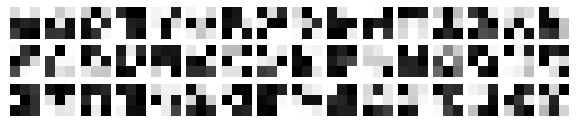
\includegraphics[width=0.8\textwidth]{Filters_after}
            \caption{Filters after training}
        \end{subfigure}
        \caption{Filters at different times}
    \end{figure}

    \subsection{Comment on the evolution of the filters}

    Firstly, when the filters were initialised they were done so randomly, so there doesn't seem like there is a particular pattern. As the model trains, the filters don't change drastically, it instead does so slowly. Some filters haven't even changed at all from the initial point right until the end. This would point towards the model adapting the current filters and tweaking them, where any filters that already have a recognisable pattern stay the same. One of the filters in my example looks like an 'n' and it stays so throughout the experiment.\\

    \section{Part III: Visualising Features}

    \subsection{Results}
    \begin{figure}[h!]
        \centering
        \begin{subfigure}[t]{0.6\textwidth}
            \centering
            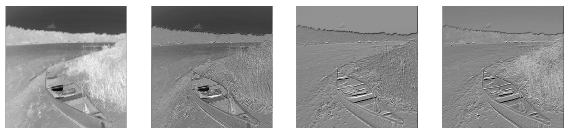
\includegraphics[width=0.6\textwidth]{image1_layer1}
            \caption{First layer}
            \label{pic1}
        \end{subfigure}
        \begin{subfigure}[t]{0.6\textwidth}
            \centering
            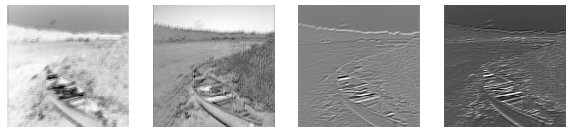
\includegraphics[width=0.6\textwidth]{image1_layer2}
            \caption{Second layer}
        \end{subfigure}
        \begin{subfigure}[t]{0.6\textwidth}
            \centering
            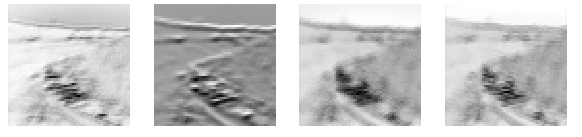
\includegraphics[width=0.6\textwidth]{image1_layer3}
            \caption{Third layer}
        \end{subfigure}
        \caption{Features of the first image}
    \end{figure}

    \begin{figure}[h!]
        \centering
        \begin{subfigure}[t]{0.6\textwidth}
            \centering
            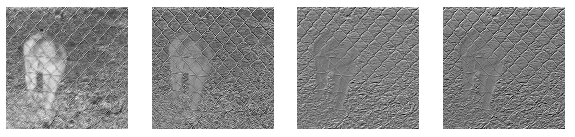
\includegraphics[width=0.6\textwidth]{image2_layer1}
            \caption{First layer}
        \end{subfigure}
        \begin{subfigure}[t]{0.6\textwidth}
            \centering
            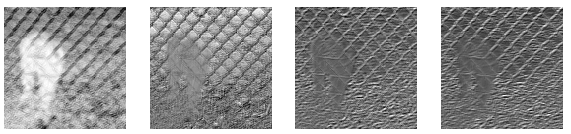
\includegraphics[width=0.6\textwidth]{image2_layer2}
            \caption{Second layer}
        \end{subfigure}
        \begin{subfigure}[t]{0.6\textwidth}
            \centering
            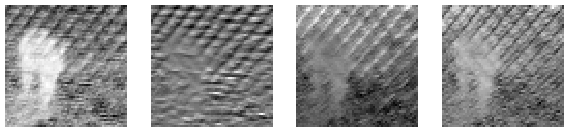
\includegraphics[width=0.6\textwidth]{image2_layer3}
            \caption{Third layer}
        \end{subfigure}
        \caption{Features of the second image}
    \end{figure}

    \subsection{Comment on the evolution of the features}
    Once the best model from the previous part has been trained, I have forwarded an image, to see how the image gets transformed over the layers. In the first layer, you can see that the model tries to separate the background from the object. In both figures first picture from the left, you can see that the boat/cat is clearly highlighted, where in the other pictures, the focus is more on the backgrounds, and how the different objects are separated. The first 2 of images on the left seem to have a lot of detail too, but as you go to the right, the detail is lost. This is especially true for the second image with the cat, where 2 of the pictures look close to identical, and the foreground blends with the background.\\

    As you go down the layers, the images get more blurry, which is expected since the images will get smaller and smaller. Alongside getting blurry, the images also increasingly lose detail, but they seem to lose detail in the background not in the foreground. This can be seen with the cat, as it looks like it is zooming in on the cat as you go down the layers.\\
    
    However, the cat on by the third layer looks like a giant round blur. Although, the model is still being able to track where it is, which is tricky in this image since there is a metal net between the cat and camera. The boat on the other hand seems to be being coloured in black where the boat is. In the first layer, only a particularly dark part of the boat is in black, then by the third layer, almost half the boat is coloured in black.\\


    \section{Part IV: Experimenting with Network}


    \subsection{Change 1: Different Kernel Sizes}

    \subsubsection{Experiments Made}

    The first change I have made do the model, is to tweak the kernel sizes both in the max pool layer as well as convolutional layer. The model seem to favour smaller kernel sizes for the convolutional layers, though it could be partially attributed to the fact that max pool operation can be replaced by a larger stride in the convolutional layers \cite{maxpoolrep}. So I have decided to drop max pooling, but increase the stride by two. The effect of that wasn't as expected, and I did not receive results similar to the paper. Performance has dropped to 41\% on unseen data as seen on the confusion matrix.\\

    \begin{figure}[h!]
        \centering
        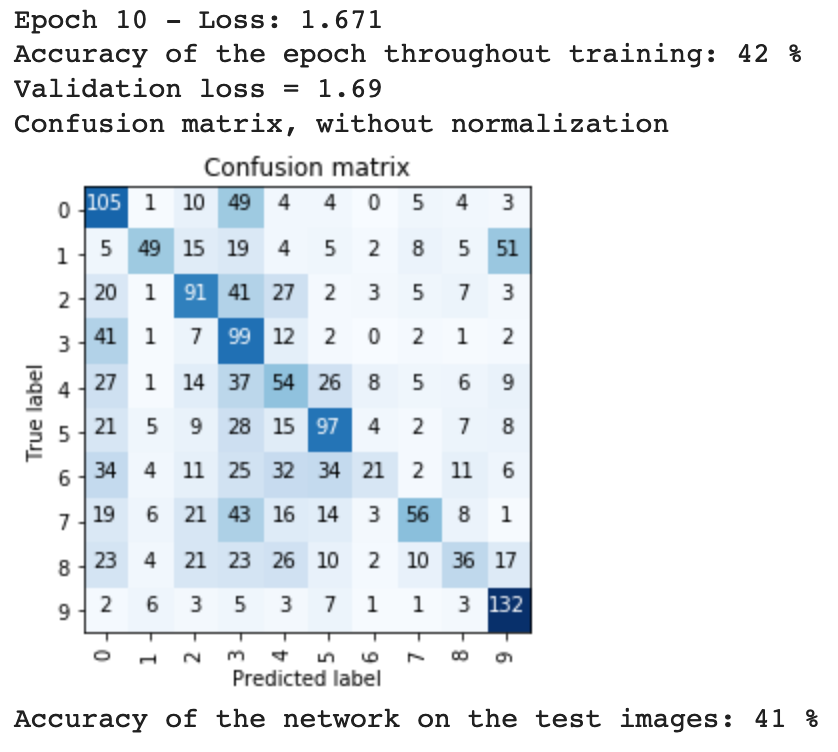
\includegraphics[width=0.5\textwidth]{first_final}
        \caption{Removal of Max Pool}
    \end{figure}

    Next, seeing as the filters from the first layer have not been tested, I have decided to test different sizes of its kernel. I believed that would work as the features from the first layer seem to be extremely important and set the precedent for the following layers. Furthermore, the lower kernel sizes of the previous layers could benefit from having to extract smaller features from a bigger size of features. In conjunction with that I decided to also increase max pooling size and kernel size to 3 to balance it out, similarly to GoogleNet \cite{googlenet}. The experiment lead to 42\% accuracy and overall worse model. As seen by the confusion matrix.\\

    \begin{figure}[h!]
        \centering
        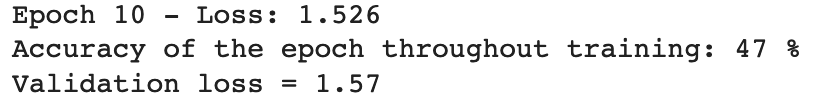
\includegraphics[width=0.5\textwidth]{7ks_3mp_train}
        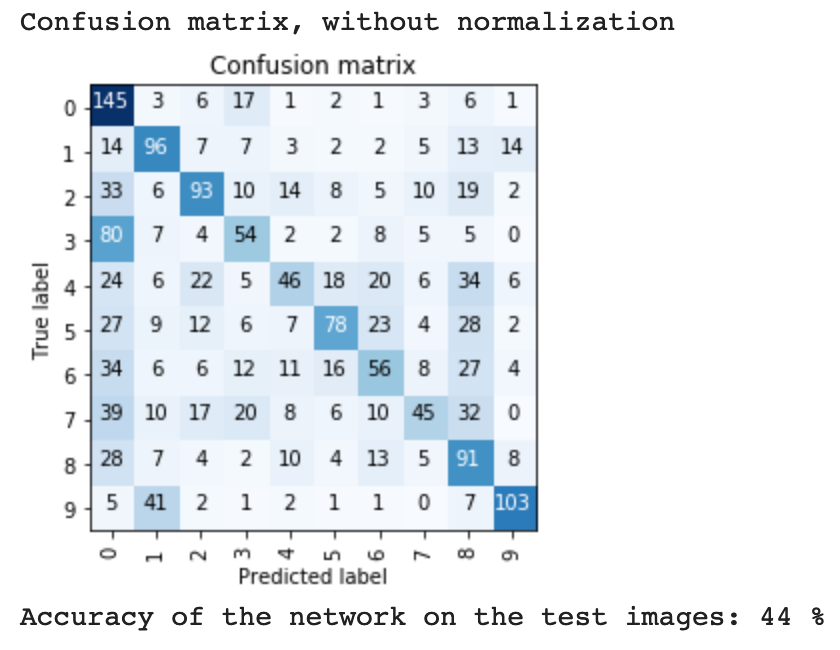
\includegraphics[width=0.5\textwidth]{7ks_3mp}
        \caption{Increasing Kernel and Max Pool}
    \end{figure}

    \subsection{Change 2: Different Output Features}

    I have then decided that changing the size of the convolutional kernel or max pool on it's own won't be beneficiary. Therefore, I have decided to change the output features and input features of all the convolutional layers. I have chosen the following parameters for each layer: first convolutional layer (input size = 3, output size = 32, kernel size = 3), second convolutional layer (input size = 32, output size = 64, kernel size = 5), first convolutional layer (input size = 64, output size = 128, kernel size = 5). I have also set all the max pools size of (3,3) and stride of 2. The increase in kernel size and max pool was due to the increased number of outputs. Once through the last layer, the flattened outputs reached dimensions of $100,000$, which was huge. Hence, I used larger pools to reduce the size of these dimensions. The overall effect of that was much more positive rising the accuracy of the model to 53\%.

    \begin{figure}[h!]
        \centering
        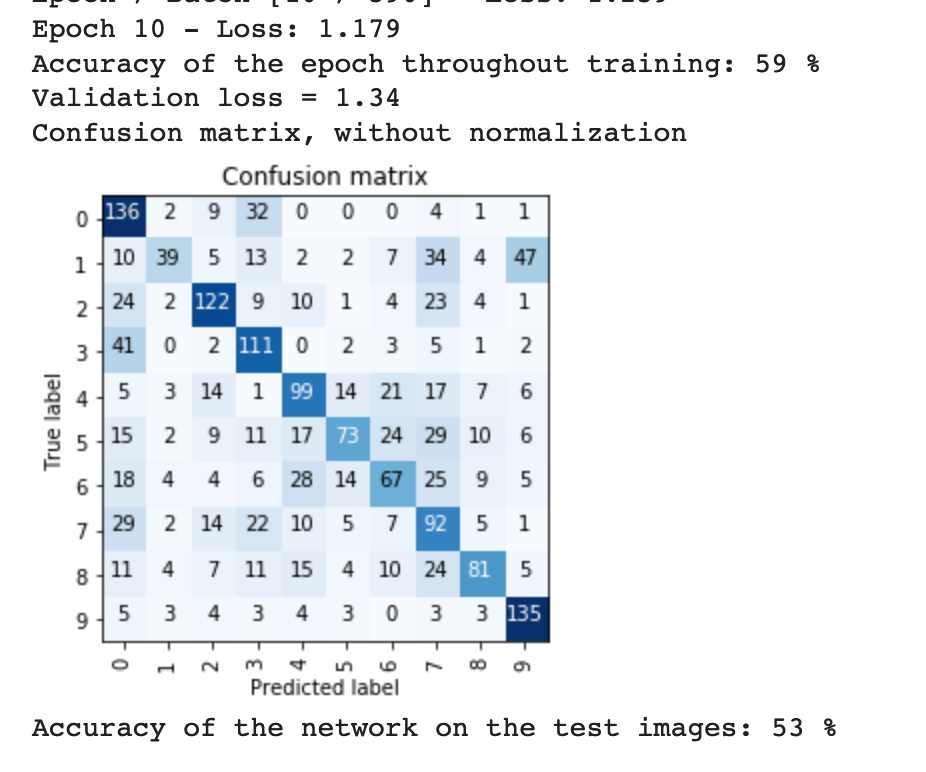
\includegraphics[width=0.5\textwidth]{bigger_output}
        \caption{Increasing Output features}
    \end{figure}

    \subsection{Change 3: Different optimizer}

    \subsection{Change 4: More Epochs}


    \subsection{Result}
    The final result of my network is as following

    \bibliographystyle{abbrv}
    \bibliography{ref}
\end{document}